%!TEX root = ./template-skripsi.tex
%-------------------------------------------------------------------------------
%                            BAB III
%               			PEMBAHASAN
%-------------------------------------------------------------------------------

\chapter{IMPLEMENTASI PROGRAM}

Dalam mengembangkan perangkat lunak ini, penulis menggunakan model Spiral seperti yang telah tertera pada \emph{System Development Life Cycle}. Tahapan-tahapannya antara lain adalah identifikasi masalah, pembangunan rancangan (desain), implementasi kode, dan evaluasi sistem.



\section{Identifikasi Masalah}

Penulis melakukan wawancara dengan perwakilan opmawa pada tanggal 22 April 2019 dan pada tanggal 20 Mei 2019. Dari hasil wawancara tersebut diperoleh hasil sebagai berikut: 

\begin{enumerate}
	\item Penyebaran informasi mengenai segala bentuk kegiatan atau program kerja dilakukan di media sosial Whatsapp, Instagram, dan Line.
	
	\item Berkas pada umumnya disimpan di penyimpanan internal gawai anggota yang bersangkutan.
\end{enumerate}

Dari wawancara yang telah dilakukan, ditemukan beberapa kendala yang sering dialami oleh opmawa selama proses pelaksanaan program kerja. Kendala-kendala tersebut antara lain:

\begin{enumerate}
	\item Informasi penting melalui pesan hilang karena pesan yang diberikan telah tertimbun oleh pesan lainnya.
	
	\item Pengarsipan dokumen yang belum baik sehingga memengaruhi kinerja pelaksanaan program kerja.
	
	\item Terjadinya \emph{miss communication} jika ada agenda untuk melakukan kumpul/ rapat bersama.
	
	\item Beberapa anggota ada yang tidak/ kurang mengetahui rencana program kerja yang telah di rencanakan beserta prosesnya.
	
	\item Anggota kepengurusan periode saat ini, ada yang tidak mengetahui mengenai pencapaian/ evaluasi dari tahun kepengurusan periode sebelumnya.
\end{enumerate}

Bersadarkan permasalahan tersebut penulis memberikan usulan mengenai perangkat lunak yang akan dikembangkan antara lain:

\begin{enumerate}
	\item Aplikasi dibuat dengan dua \emph{user} yaitu Badan Eksekutif Mahasiswa (BEM) dan Badan Perwakilan Mahasiswa (BPM).
	
	\item BEM dapat mengelola hal-hal yang berkaitan dengan pelaksanaan program kerja maupun pendaftaran kabinet kepengurusan.
	
	\item BPM dapat mengelola program kerja yang dilakukan oleh BPM dan dapat memberikan penilaian terhadap program kerja yang dilakukan oleh BEM.
\end{enumerate}

\section{Pembangunan Perancangan (Desain)}

Pada tahap ini penulis akan merepresentasikan gambaran dan kebutuhan sistem melalui bentuk komunikasi visual berupa \emph{use case diagram}, \emph{entity relationship database}, \emph{activity diagram}, dan \emph{user interface}.

\subsection{Diagram \emph{Use Case}}
\emph{User} pada aplikasi ini terdiri dari dua lembaga yaitu Badan Eksekutif Mahasiswa (BEM) dan Badan Perwakilan Mahasiswa (BPM). Adapun hal-hal yang dapat dilakukan oleh BEM antara lain:

\begin{enumerate}
	\item Mengubah profil BEM.
	\item Kelola registrasi sistem (prodi, jabatan, kabinet).
	\item Kelola keanggotaan BEM.
	\item Kelola program kerja BEM.
	\item Kelola kepanitiaan program kerja.
	\item Kelola berkas BEM.
	\item Kelola pembagian tugas dalam program kerja.
	\item Kelola keuangan. 
	\item Kelola evaluasi program kerja.
	\item Kelola agenda rapat.	
\end{enumerate}

Berikut adalah hal-hal yang dapat dilakukan oleh BPM antara lain:

\begin{enumerate}
	\item Mengubah profil BPM.
	\item Kelola keanggotaan BPM.
	\item Kelola program kerja BPM.
	\item Kelola anggota komisi pada divisi/ departemen yang didaftarkan oleh BEM.
	\item Kelola berkas BPM.
	\item Kelola agenda rapat.
	\item Mengisi penilaian pada program kerja yang dilaksanakan oleh BEM.
	Mengisi evaluasi program kerja untuk program kerja BEM.
\end{enumerate}

Berikut adalah \emph{use case diagram} yang dapat digambarkan dari berbagai fitur yang telah disebutkan dari aplikasi sistem informasi manajemen program kerja :

\begin{figure}[H]
	\centering
	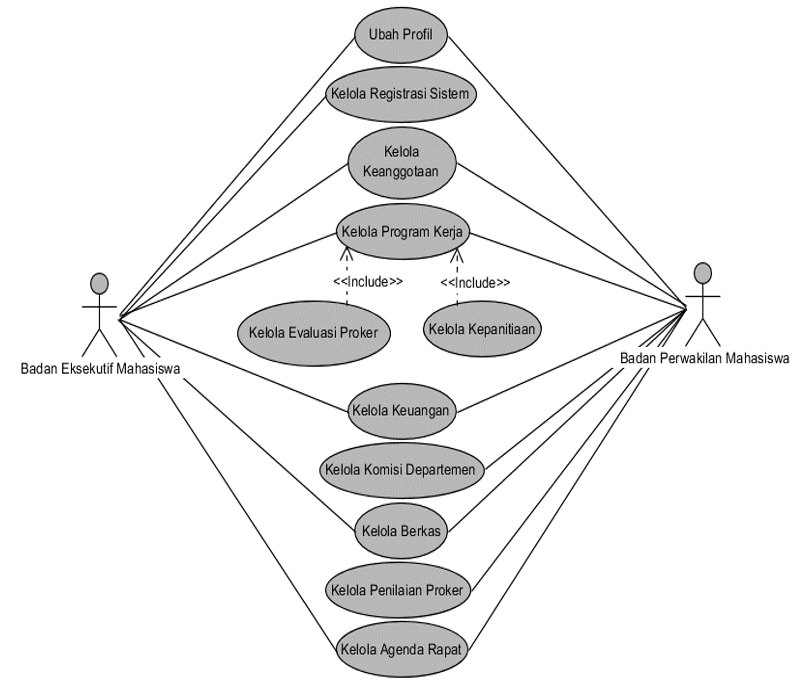
\includegraphics[width=1.0\textwidth]{gambar/usecase}
	\caption{Desain \emph{Use Case Diagram} Sistem Informasi Manajemen}
	\label{usecase_diagram}
\end{figure}

Pada sistem ini, BEM dapat mengelola data registrasi pada sistem seperti data mengenai daftar Program Studi dan daftar nama departemen yang ada pada periode kepengurusan. Sedangkan BPM dapat mengelola program kerja dan memberikan penilaian terhadap program kerja BEM yang telah terlaksana.

\subsection{\emph{Entity Relationship Diagram}}

ERD pada aplikasi ini berfungsi sebagai gambaran desain \emph{database} beserta relasi-relasi antar tabel. Penulis membuat desain \textit{database} yang terdiri dari 14 (empat belas) tabel yang saling berintegrasi. Tabel-tabel tersebut digunakan untuk menyimpan data mengenai data \textit{user}, keuangan, program kerja, kepanitiaan, pemberkasan, dan agenda rapat.

\begin{figure}[H]
	\centering
	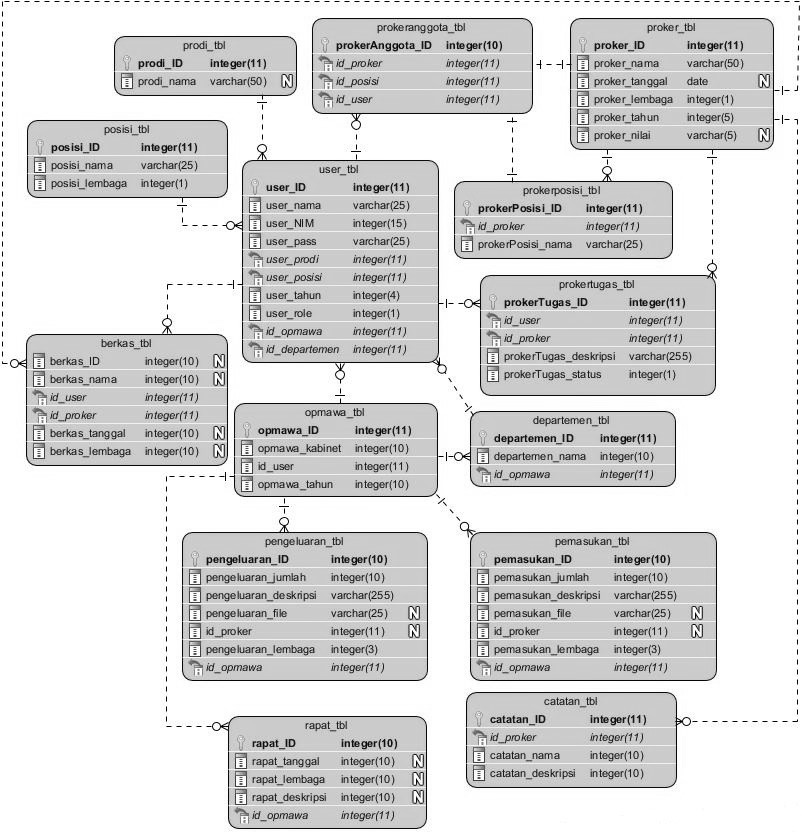
\includegraphics[width=1.0\textwidth]{gambar/erd}
	\caption{Desain \emph{Entity Relationship Diagram} Sistem Informasi Manajemen}
	\label{entityrelationship_diagram}
\end{figure}

\subsection{\textit{Class Diagram}}

\textit{Class diagram} pada aplikasi sistem informasi manajemen program kerja terdiri dari 10 (sepuluh) \textit{class} yang saling terhubung. \textit{Class user} yang menyimpan metode untuk \textit{login} atau \textit{logout}. \textit{Class user} merupakan generalisasi dari dua \textit{class} lainnya yaitu \textit{class} Badan Legislatif dan \textit{class} Badan Eksekutif. \textit{Class} program kerja berfungsi untuk menyimpan metode pendataan program kerja. \textit{Class} kepanitiaan merupakan \textit{class} yang tidak dapat berdiri sendiri tanpa adanya \textit{class} program kerja. \textit{Class} lembaga merupakan bagian dari \textit{class user} dan program kerja. \textit{Class} berkas, catatan, dan keuangan memiliki relasi dengan \textit{class} lembaga dan adakalanya dibutuhkan oleh \textit{class} program kerja. Dan yang terakhir adalah \textit{class} jadwal rapat yang berfungsi sebagai jadwal agenda rapat oleh \textit{user}.

\begin{figure}[H]
	\centering
	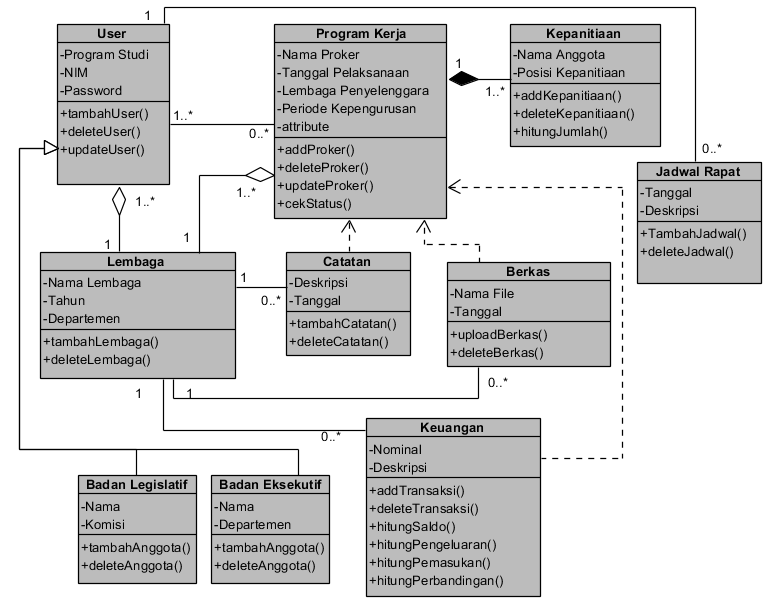
\includegraphics[width=1.0\textwidth]{gambar/class}
	\caption{Desain \emph{Class Diagram} Sistem Informasi Manajemen}
	\label{class_diagram}
\end{figure}


\subsection{\textit{Activity Diagram}}

\textit{Activity diagram} pada aplikasi sistem informasi manajemen program kerja opmawa meliputi alur pendaftaran anggota, pendaftaran program kerja dan kepanitiaannya, pencatatan keuangan program kerja/ umum, dan registrasi sistem. Berikut gambaran beberapa desain visual untuk \textit{activity diagram} aplikasi sistem informasi manajemen program kerja :

\begin{figure}[H]
	\centering
	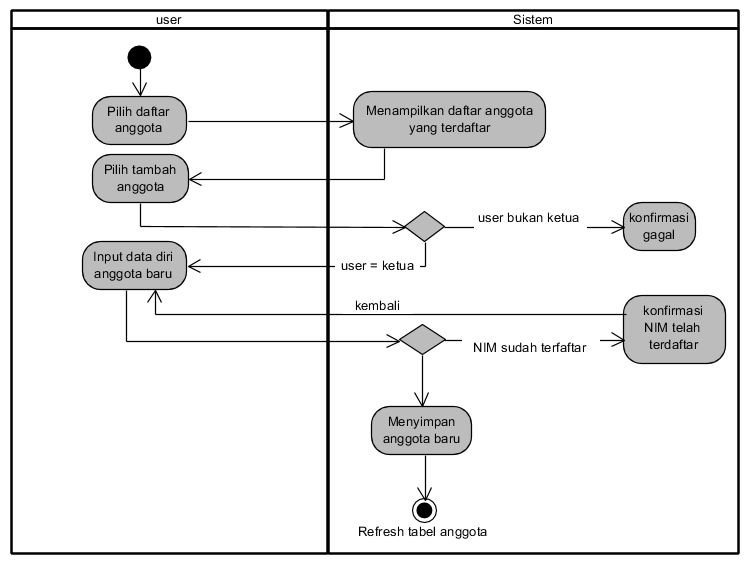
\includegraphics[width=1.0\textwidth]{gambar/Activitytambahanggota}
	\caption{Desain \emph{Activity Diagram} Pendaftaran Anggota}
	\label{activityAnggota_diagram}
\end{figure}

Pada alur pendaftaran anggota, hanya ketua dari masing-masing lembaga (eksekutif/ legislatif) yang dapat mendaftarkan anggota nya. Ketua mendaftarkan anggota baru dengan mengisi \textit{form} pendaftaran, kemudian sistem akan melakukan pemeriksaan. Apabila NIM (Nomor Induk Mahasiswa) sudah terdaftar dan NIM yang terdaftar tersebut memiliki data periode kepanitiaan yang sama dengan ketua, maka sistem akan otomatis menolak dan mengarahkan untuk mengisi ulang \textit{form}. Jika NIM belum terdaftar, maka data akan tersimpan dalam \textit{database}.


\begin{figure}[H]
	\centering
	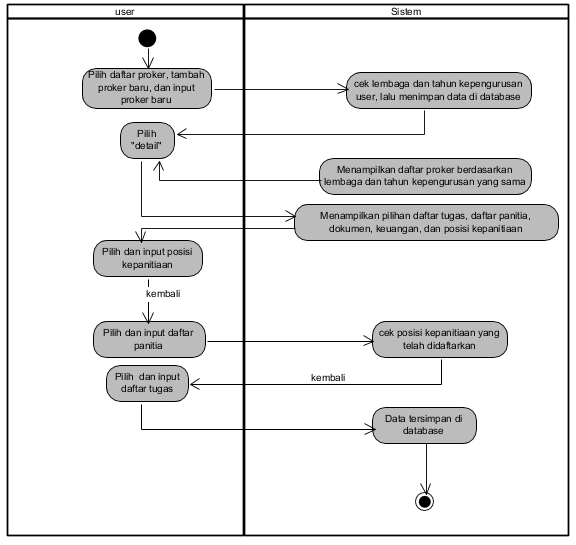
\includegraphics[width=1.0\textwidth]{gambar/Activityproker}
	\caption{Desain \textit{Activity Diagram} Pendaftaran Program Kerja Dan Kepanitiaannya}
	\label{activityProker_diagram}
\end{figure}

Pada alur pendaftaran program kerja dan kepanitiaannya, \textit{user} meng-\textit{input} nama program kerja beserta rencana tanggal pelaksanaannya. Pada kolom tanggal dapat dikosongkan terlebih dahulu. Setelah mengisi \textit{form}, sistem akan mengambil beberapa data dari \textit{user} untuk mengklasifikasikan program kerja berdasarkan periode kepengurusan dan lembaganya. Setelah berhasil, \textit{user} dapat memilih secara bebas untuk mengelola data dari program kerja. 

\textit{User} dapat terlebih dahulu mendaftarkan posisi kepanitiaan yang diinginkan, kemudian mendaftarkan masing-masing anggota untuk masuk kedalam kepanitiaan dengan posisi kepanitiaan seperti yang telah terdaftar. Setelah data tersimpan, selanjutnya \textit{user} dapat mengelola data-data lainnya seperti catatan mengenai program kerja, keuangan, unduh/ unggah dokumen, dan memberikan catatan penugasan untuk setiap anggota kepanitiaan. 

\begin{figure}[H]
	\centering
	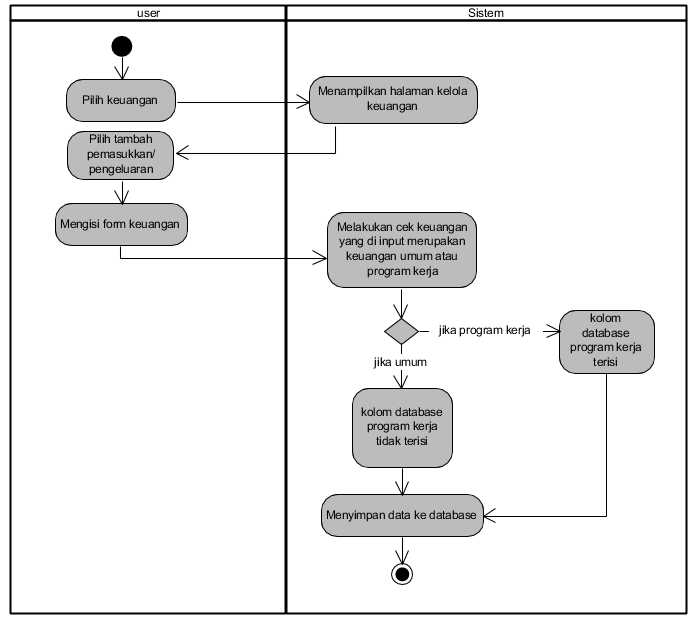
\includegraphics[width=1.0\textwidth]{gambar/Activitykeuangan}
	\caption{Desain \textit{Activity Diagram} Kelola Keuangan}
	\label{ActivityKeuangan_diagram}
\end{figure}

Alur keuangan terbagi atas 2 jenis kelola keuangan yaitu kelola keuangan umum dan kelola keuangan yang berkaitan dengan pelaksanaan program kerja. \textit{User} dapat mengelola keuangan melalui \textit{menu side bar} untuk mengelola keuangan umum/ program kerja dan pada halaman detail program kerja untuk mengelola keuangan program kerja.

\begin{figure}[H]
	\centering
	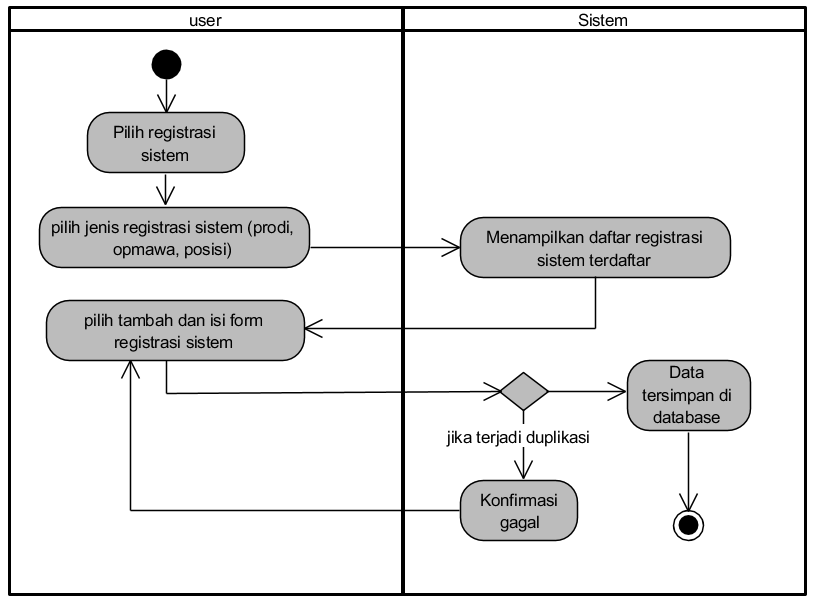
\includegraphics[width=1.0\textwidth]{gambar/Activitysistem}
	\caption{Desain \textit{Activity Diagram} Registrasi Sistem}
	\label{ActivitySistem_diagram}
\end{figure}

Registrasi sistem terdiri dari 3 jenis yaitu registrasi Program Studi, registrasi opmawa, dan registrasi posisi. Registrasi ini sebagai salah satu sekaligus pelengkap parameter \textit{input} pada \textit{form} yang membutuhkan data tertentu.

Registrasi Program Studi untuk mendaftarkan Program Studi yang ada di FMIPA, registrasi opmawa untuk mendaftarkan periode kepengurusan opmawa berikutnya, dan registrasi posisi untuk menentukan posisi-posisi atau struktur organisasi yang diperlukan dalam menjalani organisasi di opmawa.


\subsection{Desain \textit{Interface}}

Pada tampilan awal \textit{login} sebagai anggota BEM, terdapat pilihan untuk mendaftarkan anggota, daftar program kerja, kelola keuangan, kelola berkas/ dokumen, daftar agenda rapat, dan registrasi sistem. Berikut adalah desain untuk tampilan pada halaman BEM :

\begin{figure}[H]
	\centering
	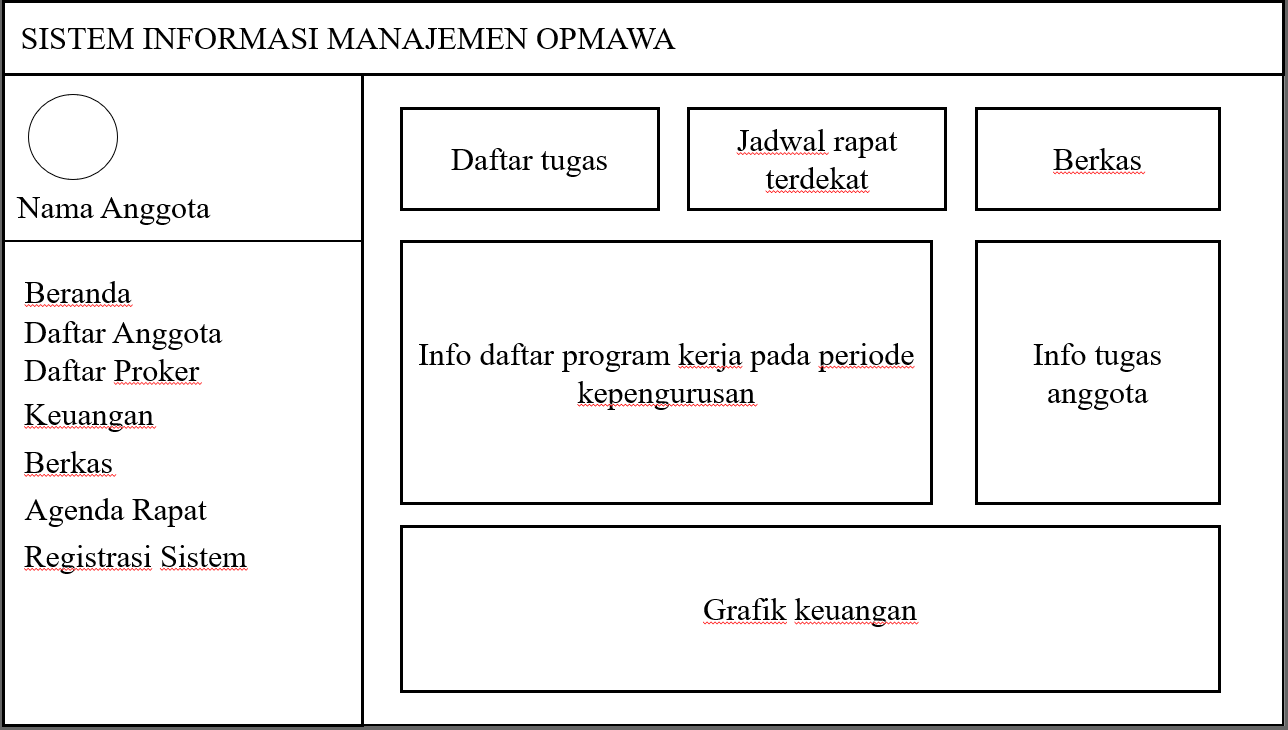
\includegraphics[width=0.9\textwidth]{gambar/tampilanberanda}
	\caption{Desain Tampilan Awal / Beranda}
	\label{Tampilan_beranda}
\end{figure}

Gambar 3.8 menampilkan gambaran desain untuk tampilan setelah \textit{login} sebagai anggota BEM. Pada tampilan awal ini, \textit{user} dapat melihat daftar pilihan dan tampilan informasi seperti daftar tugas, informasi mengenai program kerja yang akan dilaksanakan pada periode kepengurusan yang sesuai dengan \textit{user}, info tugas yang diberikan oleh \textit{user}, dan grafik keuangan yang di bagi berdasarkan pemasukan dan pengeluaran dari masing-masing program kerja yang telah terdaftar.


\begin{figure}[H]
	\centering
	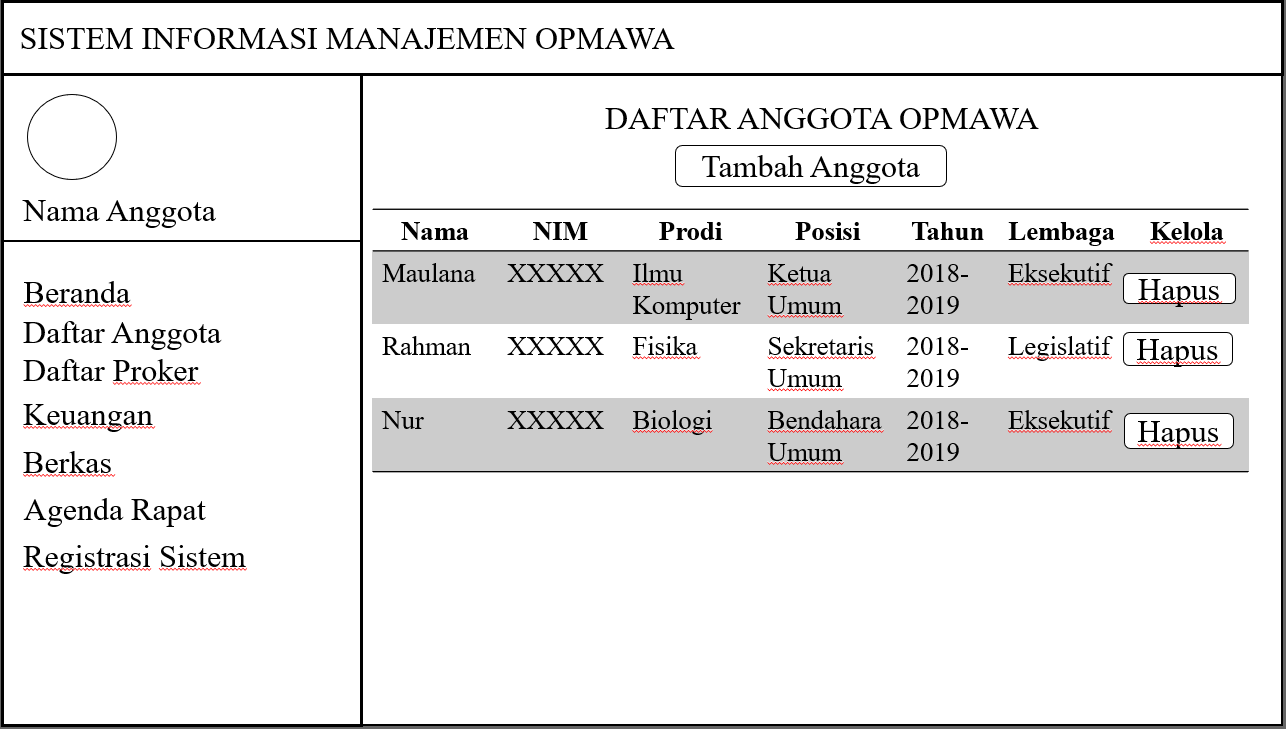
\includegraphics[width=0.9\textwidth]{gambar/tampilananggota}
	\caption{Desain Tampilan Daftar Anggota opmawa}
	\label{Tampilan_anggota}
\end{figure}

Gambar 3.9 merupakan desain tampilan daftar anggota yang telah terdaftar untuk periode kepengurusan tertentu. Di tampilan ini, \textit{user} yang berada pada posisi ketua lembaga juga memungkinkan untuk mendaftarkan anggota baru atau menghapus anggota lama. Ketua lembaga hanya dapat mengelola daftar anggota yang berada pada lembaga yang sama.

\begin{figure}[H]
	\centering
	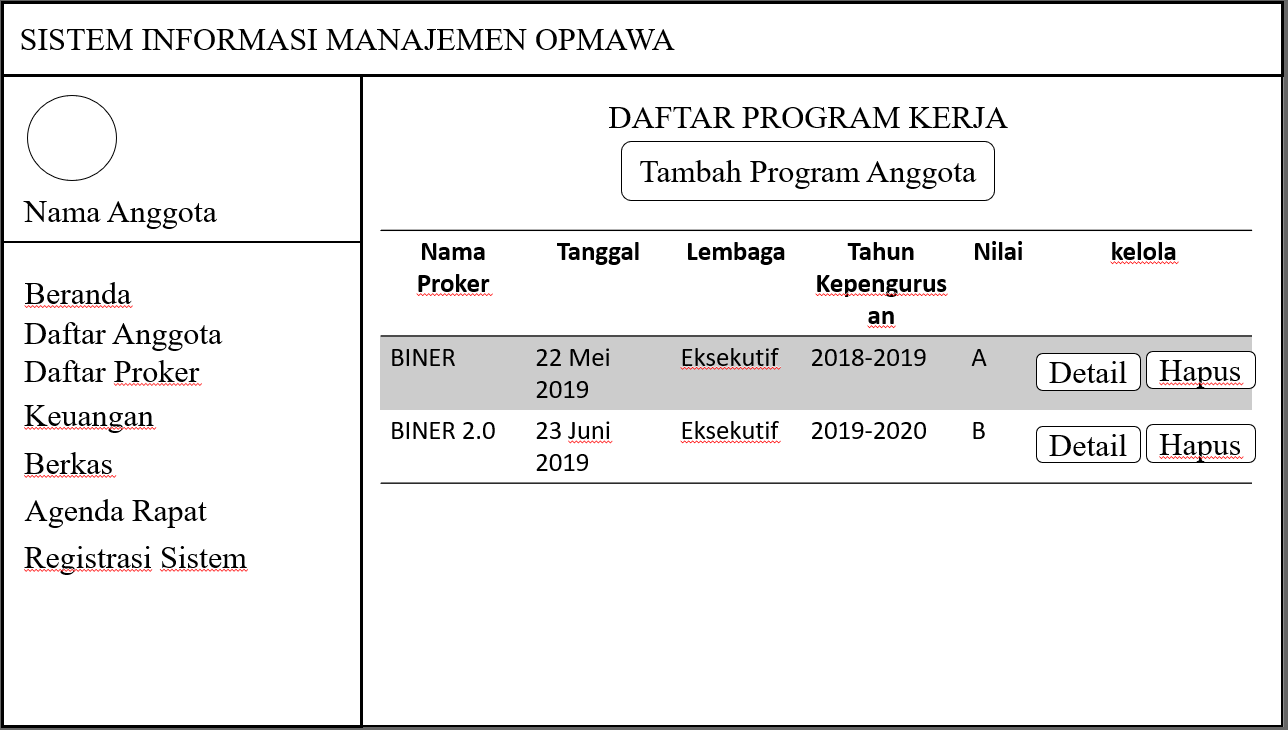
\includegraphics[width=0.9\textwidth]{gambar/tampilanproker}
	\caption{Desain Tampilan Daftar Program Kerja}
	\label{Tampilan_proker}
\end{figure}

Gambar 3.10 merupakan desain tampilan daftar program kerja yang telah direncanakan dan didaftarkan pada periode yang sesuai dengan tahun kepengurusan \textit{user} yang mendaftarkannya. \textit{User} juga dapat melihat informasi lebih mengenai program kerja dengan memilih opsi detail. Pada kolom "Nilai" hanya akan terisi apabila tanggal pelaksanaan program kerja telah terlewati dan diisi oleh lembaga legislatif.

\begin{figure}[H]
	\centering
	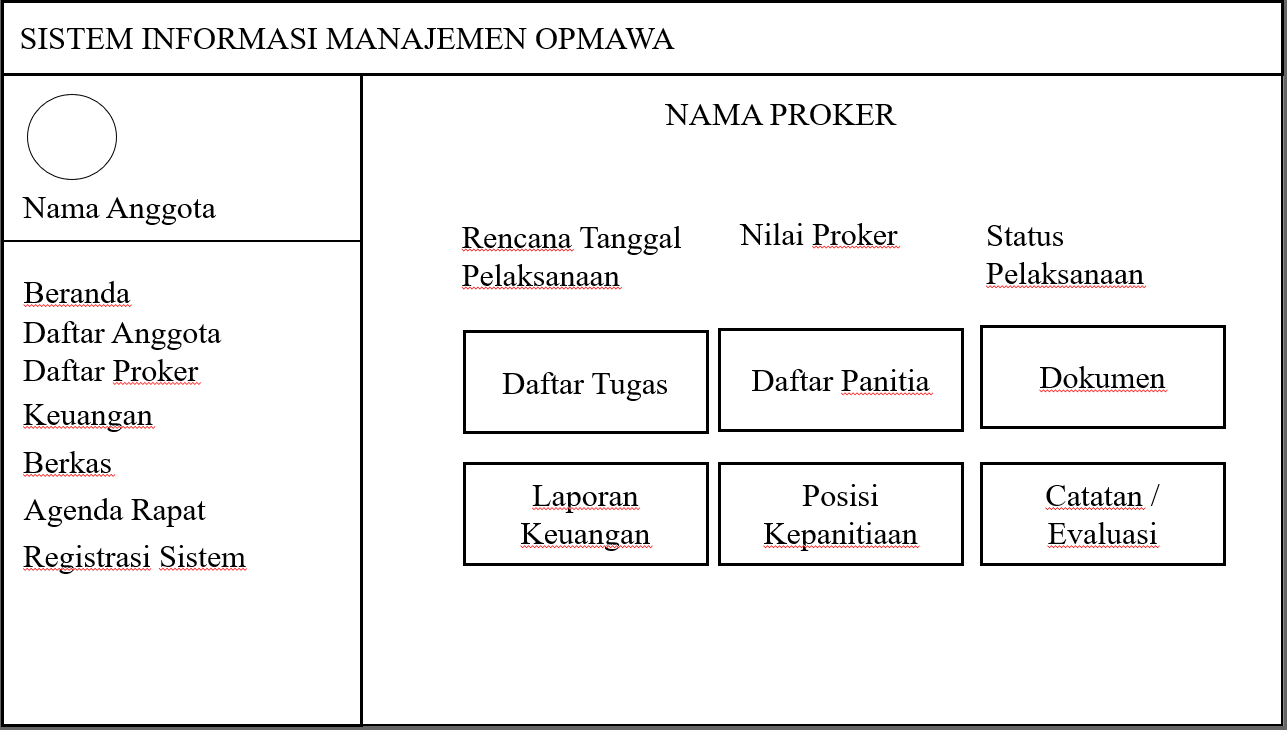
\includegraphics[width=0.9\textwidth]{gambar/tampilandetailproker}
	\caption{Desain Tampilan Detail Program Kerja}
	\label{Tampilan_detail_proker}
\end{figure}

Gambar 3.11 merupakan desain tampilan detail program kerja yang terdaftar. Pada tampilan ini memungkinkan \textit{user} untuk melihat tanggal pelaksanaan dan penilaian program kerja apabila telah selesai terlaksana, mengelola data-data dan keperluan lainnya pada suatu program kerja seperti mendaftarkan posisi kepanitiaan, mendaftarkan anggota opmawa yang akan terlibat dalam kepanitiaan, laporan keuangan, daftar-daftar tugas atau hal yang perlu dilakukan saat menjalankan program kerja, unduh atau unggah dokumen, dan catatan-catatan lainnya yang sekiranya diperlukan sebagai catatan maupun evaluasi yang terjadi dalam pelaksanaan program kerja.